% Dominik Gothe
% Based on Marco Miani's work on "Spherical and cartesian grids"
\documentclass[12pt]{article}
\usepackage{tikz}
\usepackage{pgfplots}
\usepackage{amsmath}

%\pgfplotsset{compat=1.9}
%\usetikzlibrary{calc,fadings,decorations.pathreplacing}
\tikzset{ >=latex } % Prettier Arrows
%% helper macros

\def\R{5} 			% Radius of Sphere
\def\D{5} 			% Distance to Project outside of Sphere
\def\tilt{25} 		% Tilt of Sphere
\def\zeroAz{-100}	% Zero Azimuth Reference Line
\def\leftLong{-25} 	% Longitude of point P
\def\midLong{-40}
\def\rightLong{-55} % longitude of point Q
\def\lowLat{30}  	% Low Latitude of FOV
\def\midLat{45}  	% Center Latitude
\def\highLat{60} 	% High Latitude of FOV



\newcommand\pgfmathsinandcos[3]{%
	\pgfmathsetmacro#1{sin(#3)}%
	\pgfmathsetmacro#2{cos(#3)}%
}
% Macro to define Longitudenal Planes
\newcommand\LongitudePlane[3][current plane]{
	\pgfmathsinandcos\sinEl\cosEl{#2}
	\pgfmathsinandcos\sint\cost{#3}
	\tikzset{#1/.estyle={cm={\cost,\sint*\sinEl,0,\cosEl,(0,0)}}}
}
% Macro to define Latitudenal Planes
\newcommand\LatitudePlane[3][current plane]{
  \pgfmathsinandcos\sinEl\cosEl{#2}
  \pgfmathsinandcos\sint\cost{#3}
  \pgfmathsetmacro\yshift{\cosEl*\sint}
  \tikzset{#1/.estyle={cm={\cost,0,0,\cost*\sinEl,(0,\yshift)}}}
}
% Drawing Longitudenal Circles (all Great-Circles)
\newcommand\DrawLongitudeCircle[2][1]{
    \LongitudePlane{\tilt}{#2}
    \tikzset{current plane/.prefix style={scale=#1}}
    \pgfmathsetmacro\angVis{atan(sin(#2)*cos(\tilt)/sin(\tilt))}
    \draw[current plane, thin, solid,  black] (\angVis:1) arc (\angVis:\angVis+180:1);
    \draw[current plane, thin, dashed, black] (\angVis-180:1) arc (\angVis-180:\angVis:1);
}
% Drawing Latitudenal Circles (not Great-Circles, except Horizon)
\newcommand\DrawLatitudeCircle[2][1]{
    \LatitudePlane{\tilt}{#2}
    \tikzset{current plane/.prefix style={scale=#1}}
    \pgfmathsetmacro\sinVis{sin(#2)/cos(#2)*sin(\tilt)/cos(\tilt)}
    \pgfmathsetmacro\angVis{asin(min(1,max(\sinVis,-1)))}
    \draw[current plane,thin,black] (\angVis:1) arc (\angVis:-\angVis-180:1);
    \draw[current plane,thin,dashed] (180-\angVis:1) arc (180-\angVis:\angVis:1);
}
% Draw Green Latitutdenal Planes (used to draw Horizon plane)
\newcommand\DrawLatPlane[2][\R]{
    \LatitudePlane{\tilt}{#2}
    \tikzset{current plane/.prefix style={scale=#1}}
    \pgfmathsetmacro\sinVis{sin(#2)/cos(#2)*sin(\tilt)/cos(\tilt)}
    \fill[current plane,green!100!black, opacity=.2] (0:1) arc (0:360:1);
}
% Used to draw spherical coordinate grids
% Draw a Longitudenal Line from leftLon to rightLon @ given angle
\newcommand\DrawLonGrid[2][1]{
	\LongitudePlane{\tilt}{#2}
	\tikzset{current plane/.prefix style={scale=#1}}
	\draw[current plane,thick,red] (180-\highLat:1) arc (180-\highLat:180-\lowLat:1);  
}
% Draw a Latitudenal Line from lowLat to highLat @ given angle
\newcommand\DrawLatGrid[2][1]{
    \LatitudePlane{\tilt}{#2}
    \tikzset{current plane/.prefix style={scale=#1}}
\draw[current plane,red,thick] (\rightLong:1) arc (\rightLong:\leftLong:1);
}

\pagestyle{empty}

\begin{document}
\begin{figure}[ht!]
	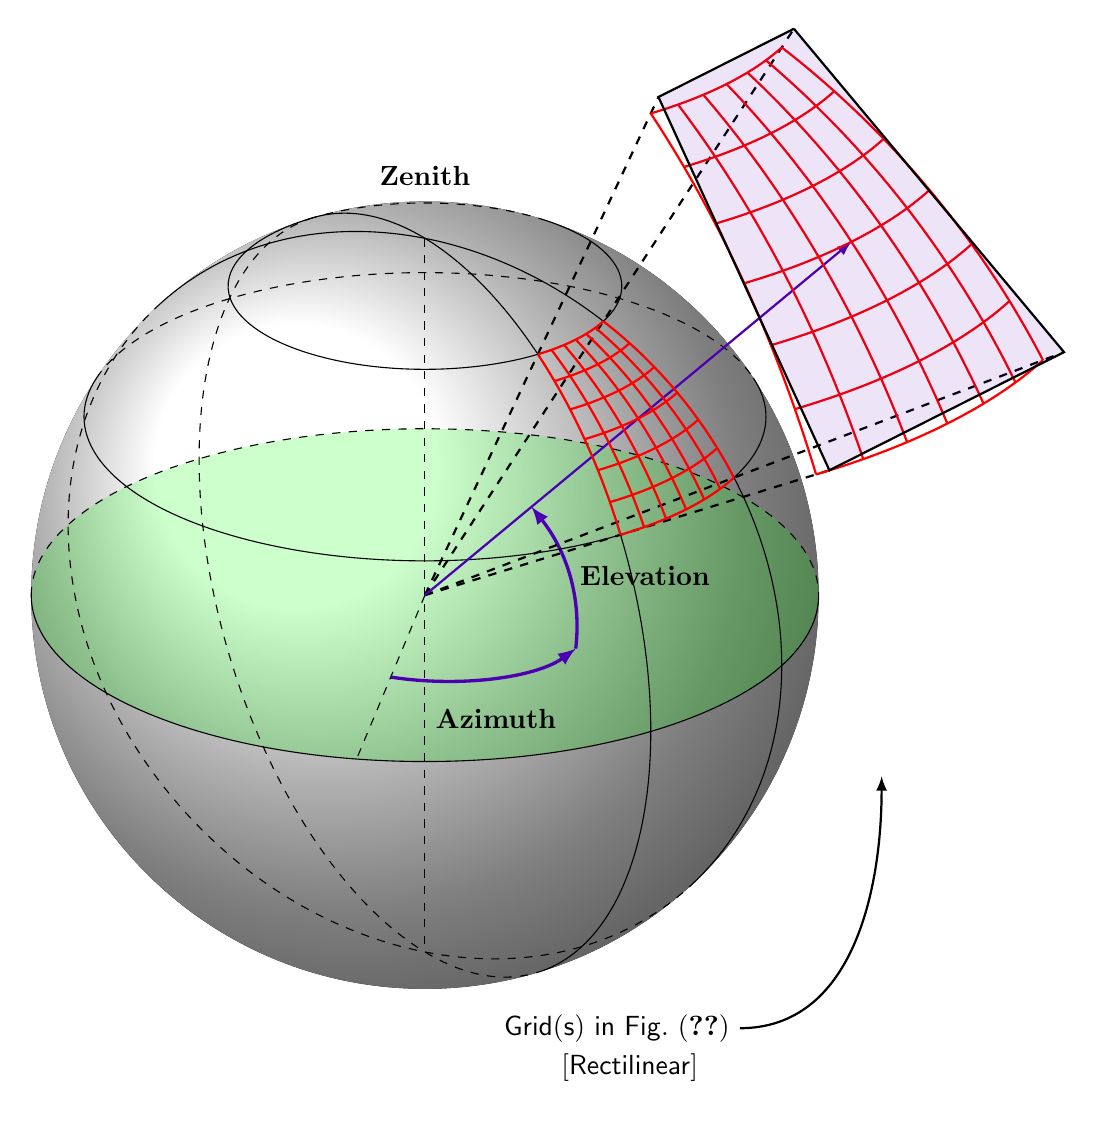
\begin{tikzpicture}[scale=1,every node/.estyle={minimum size=1cm}]   
    % Do some on-the-fly math
	\pgfmathsetmacro\H{\R*cos(\tilt)} 						% Distance to the North Pole
    \pgfmathsetmacro\DR{(\R+\D)*(2-cos(15))}				% Extra distance to elevate Rectilinear plane
	% Setup the Sphere and Horizon Plane  
    \fill[ball color=white!10] (0,0) circle (\R); 			% 3D Lighting Effect
    \DrawLatPlane[\R]{0}									% Draw the Horizon-plane
    % Define Working Planes
	\LongitudePlane[zeroAzPlane]    {\tilt}{\zeroAz}		% Zero Azimuth Plane
	\LongitudePlane[leftLongPlane]  {\tilt}{\leftLong}  	% Left Longitudenal Plane
    \LongitudePlane[centerLongPlane]{\tilt}{\midLong}		% Center Longitudenal Plane
	\LongitudePlane[rightLongPlane] {\tilt}{\rightLong} 	% Right Longitudenal Plane
    \LatitudePlane[horizonPlane]    {\tilt}{0}				% Horizon Plane (Latitudenal)
   	% Define Working Coordinates
	\coordinate (O) at (0,0);								% Origin of Sphere
	\coordinate (N) at (0,\H);				% North-Pole of Sphere
	\coordinate (S) at (0,-\H);			% South-Pole of Sphere
	\path[zeroAzPlane] (\R,0) coordinate (ZA);				% Zero Azimuth point on Horizon Plane
    \path[centerLongPlane] (\R,0) coordinate (AZ);			% Point on the Horizon corrosponding to the azimuth
	% Define Points Project outside of SPhere
	\path[rightLongPlane]  (\highLat:\DR) coordinate (TRO); % Top Right of FocalPlane projected onto Rectilinear
	\path[leftLongPlane]   (\highLat:\DR) coordinate (TLO); % Top Left of FocalPlane projected onto Rectilinear
    \path[centerLongPlane] (\midLat:\R+\D) coordinate (CO); % Center of FocalPlane projected onto Rectilinear
    \path[leftLongPlane]   (\lowLat:\DR)  coordinate (BLO); % Bottom Left of FocalPlane projected onto Rectilinear
    \path[rightLongPlane]  (\lowLat:\DR)  coordinate (BRO); % Bottom Right of FocalPlane projected onto Rectilinear
    % Draw some reference lines
    \draw[dashed] (N) -- (S);								% Connect the North and South Pole
    \draw[dashed] (O) -- (ZA);								% Draw a reference line to show where azimuth = 0 falls
%    \draw[dashed, thick] (O) -- (AZ);						% Draw a reference line corrosponding to the azimuth
        
	\draw[centerLongPlane, ->, very thick, red!30!blue] (0:0.5*\R)
    	to [bend right=30] node[midway, right, black] {$\mathbf{Elevation}$} (\midLat:0.5*\R);
    \draw[horizonPlane,    ->, very thick, red!30!blue] (\zeroAz:0.5*\R)
    	to [bend right=40] node[midway, below, black] {$\mathbf{Azimuth}$} (\midLong:0.5*\R);
    
	% Longitudenal bounds of the FOV
    \DrawLongitudeCircle[\R]{\leftLong}  			% Left Longitude Circle (great circle)
    \DrawLongitudeCircle[\R]{\rightLong} 			% Right Longitude Circle (great circle)
    % Latitudenal bounds of the FOV
    \DrawLatitudeCircle[\R]{\highLat}				% High Latitude Circle (not great circle)
    \DrawLatitudeCircle[\R]{\lowLat}				% Low Latitude Circle (not great circle)
    \DrawLatitudeCircle[\R]{0} 						% Horizon Circle
	% Project FocalPlane Defining Beams
	\draw[-, dashed, black, thick] (O) -- (TLO); 	% Top-Left corner
	\draw[-, dashed, black, thick] (O) -- (BLO); 	% Bottom-Left corner
    \draw[-, dashed, black, thick] (O) -- (BRO); 	% Bottom-Right corner
    \draw[-, dashed, black, thick] (O) -- (TRO); 	% Top-Right corner
    \draw[->, thick, red!30!blue]  (O) -- (CO);		% Actuall pointing
	% Grid on Sphere
    \foreach \t in {30,35,...,60}    { \DrawLatGrid[\R]{\t} }
	\foreach \t in {125,130,...,155} { \DrawLonGrid[\R]{\t} }
	% Grid Outside Sphere
    \foreach \t in {30,35,...,60}    { \DrawLatGrid[\R+\D]{\t} }
    \foreach \t in {125,130,...,155} { \DrawLonGrid[\R+\D]{\t} }
    % Rectilinear Grid Outside
    \fill[thick, red!30!blue, opacity=.1] (TLO) -- (BLO) -- (BRO) -- (TRO) -- (TLO);
    \draw[thick, black,       opacity=1] (TLO) -- (BLO) -- (BRO) -- (TRO) -- (TLO);
    % Some Labels
	\node[above=8pt] at (N) {$\mathbf{Zenith}$}; 	% Label the Zenith
	\draw[-latex,thick](4,-5.5)node[left]{$\mathsf{Grid(s)\ in\ Fig. \ (\ref{fig:Grid})}$} to[out=0,in=270] (5.8,-2.3);
    \draw[thick](3.6,-6)node[left]{$[\mathsf{Rectilinear}]$};
   
	\end{tikzpicture}
	\caption[cap]
    {WUts dis.}
	\label{fig:Grid}
\end{figure}

\end{document} 